\section{Analyse Comparative des Paradigmes Architecturaux de Stockage Distribu\'e}

\setlength{\parskip}{3pt}

La croissance du volume de donn\'ees a rendu les architectures centralisees insuffisantes. Les systemes distribues sont devenus la norme, mais posent un defi central : garantir un \emph{lookup} efficace, la \emph{consistency} et la \emph{fault tolerance} dans un environnement de n\oe uds peu fiables.

Dans ce projet Master, nous comparons deux architectures de reference pour le stockage distribue, basees sur des paradigmes differents :

\paragraph{1. L'architecture P2P structur\'ee (Les DHTs)}
Paradigme decentralise (architecture \emph{symmetric}) : les n\oe uds ont un role homogene et s'auto-organisent dans un \emph{overlay} structure. Nous considerons plusieurs DHT (Chord, CAN, Pastry, Kademlia) qui resolvent le \emph{lookup} en general en $O(\log N)$, avec des compromis differents entre topologie logique, latence de routage, taille des tables d'etat et r\'esilience au \emph{churn}.

\paragraph{2. L'architecture hi\'erarchis\'ee orient\'ee colonnes (Mod\`ele HBase)}
A l'oppose du P2P pur, ce paradigme suit une architecture \emph{master-worker} inspiree de Bigtable. HBase vise une coherence forte, un modele oriente colonnes/versionne, et conserve une centralisation partielle (HMaster) pour la gestion des metadonnees et des transactions, en echange de meilleures performances d'ecriture et de scan.

La suite du document presente d'abord le routage et la maintenance des DHTs, puis l'architecture interne de HBase et ses mecanismes de persistance.

\subsection{\'Etude des approches P2P structur\'ee: Les DHTs}

Cette section r\'esume les principes essentiels des \emph{Distributed Hash Tables} (DHTs) : localisation des donn\'ees, routage, gestion des n\oe uds et interfaces applicatives.

\begin{tcolorbox}[bluebox]
\textbf{R\'ef\'erence} : \textcite{DBLP:conf/p2p/WehrleGR05}.
\end{tcolorbox}

\subsubsection{Introduction au probl\`eme du Lookup}

Le probl\`eme central est le \emph{lookup problem} : o\`u stocker une donn\'ee \(D\), puis comment la retrouver dans un r\'eseau distribu\'e sans coordination centrale.
\begin{quote}
\emph{"O\`u stocker, et comment trouver un certain \'el\'ement de donn\'ee D dans un syst\`eme distribu\'e sans aucun contr\^ole ou coordination centralis\'es ?"}
\end{quote}

\begin{figure}[!ht]
	\centering
		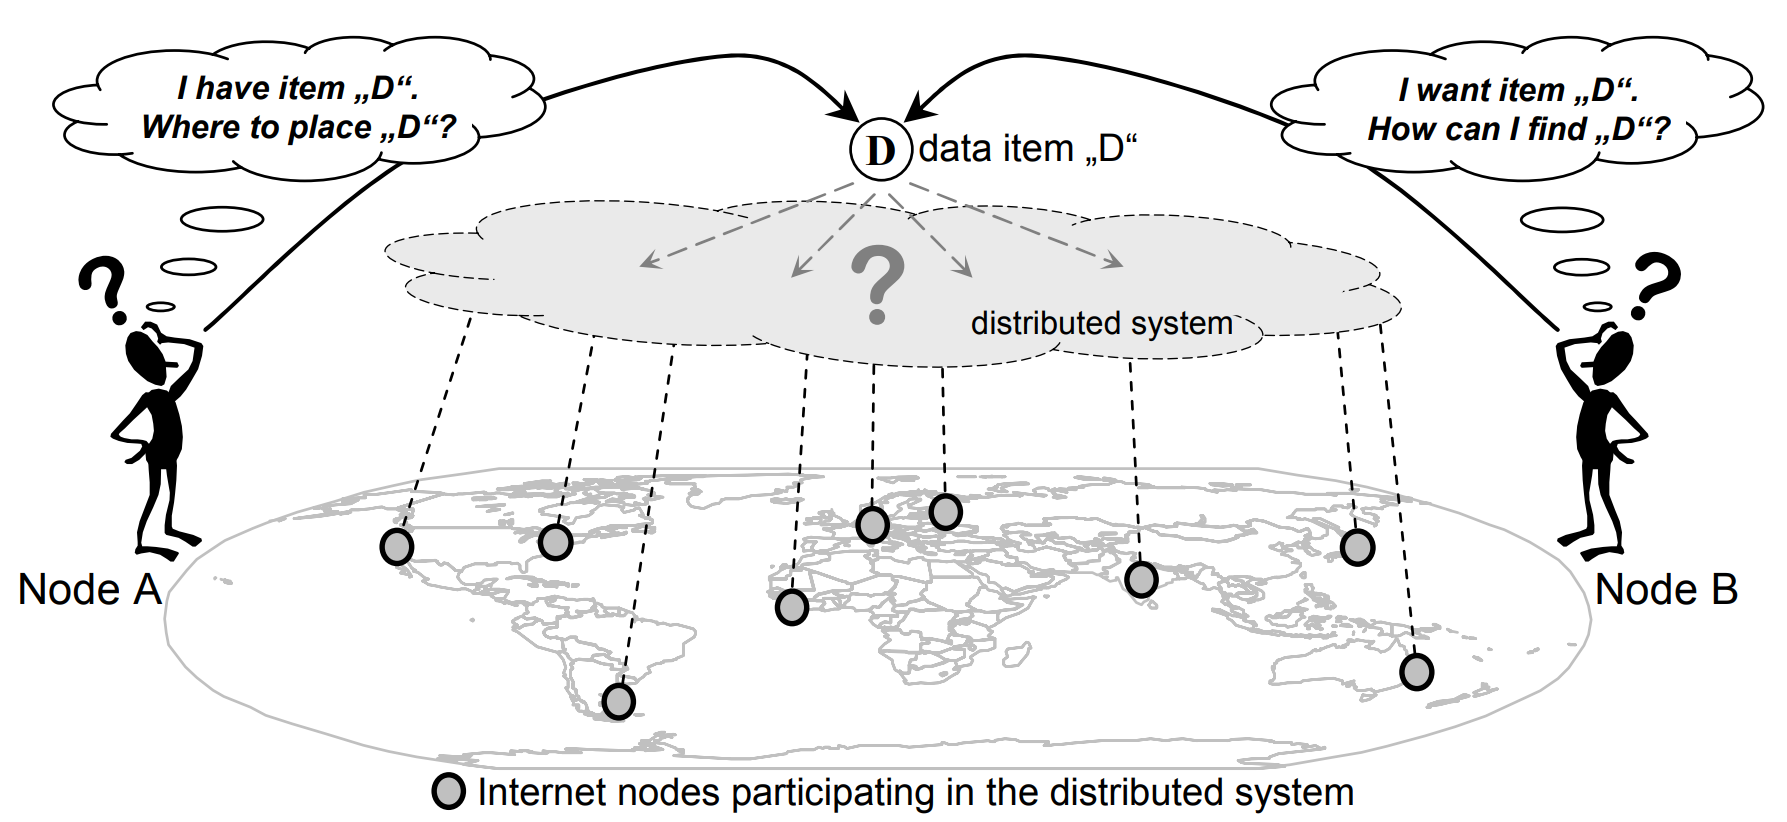
\includegraphics[width=0.7\textwidth]{images/00_lookup_problem.png}
	\caption{\textbf{Le probl\`eme du lookup} : le n\oe ud A stocke une donn\'ee \(D\) et le n\oe ud B doit la retrouver sans conna\^itre son emplacement.}
	\label{fig:00_lookup_problem}
\end{figure}

\newpage
\subsubsection{Comparaison des strat\'egies de recherche}

Trois familles de solutions sont compar\'ees.

\subsubsection*{1. Central Server}
Approche de \textbf{premi\`ere g\'en\'eration} (ex.~Napster). Un serveur central indexe les contenus. Recherche rapide en \(O(1)\), mais d\'ependance forte \`a un \emph{single point of failure}.

\begin{figure}[!ht]
	\centering
		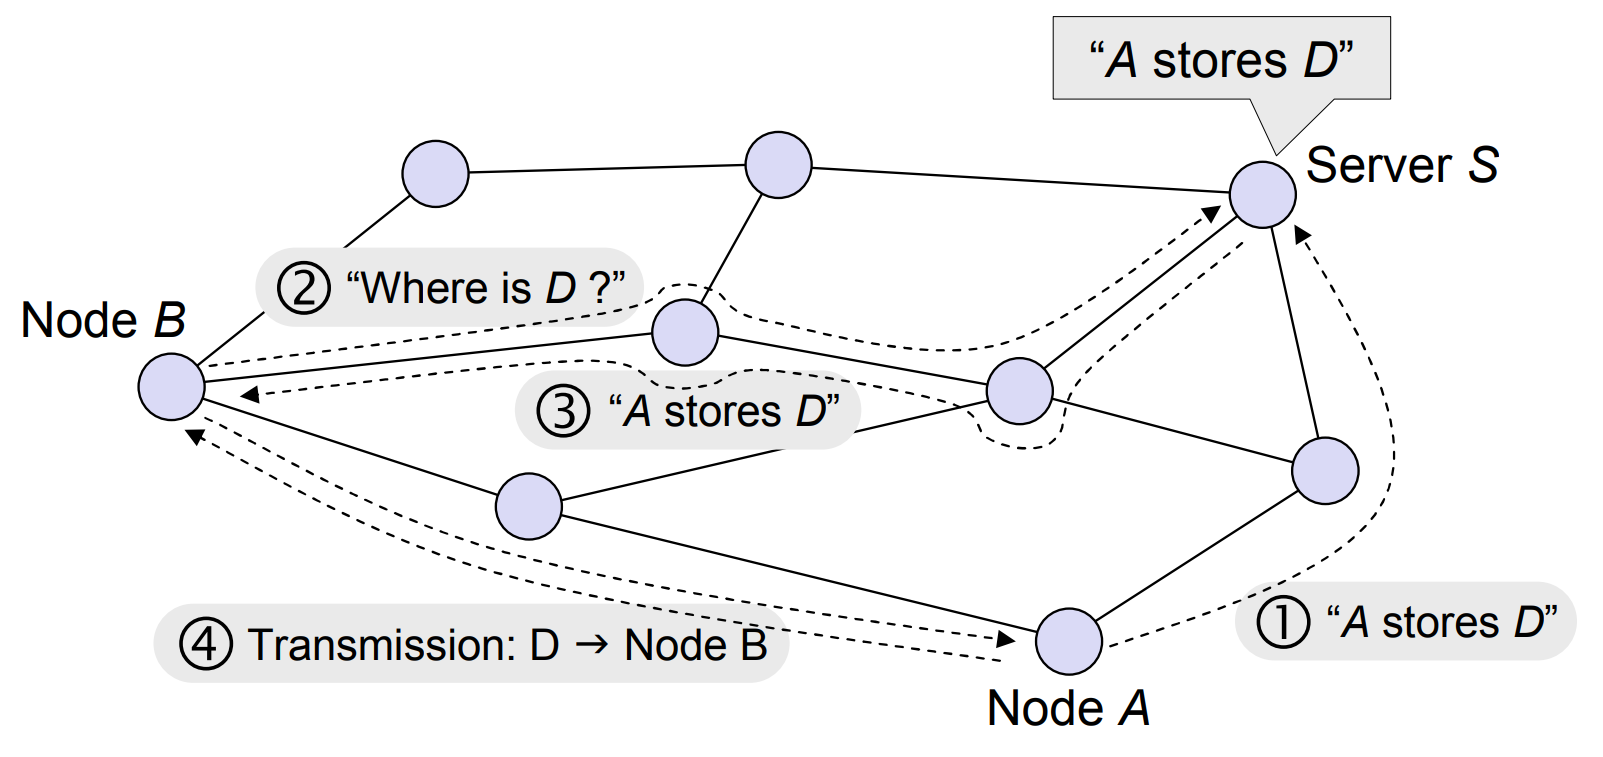
\includegraphics[width=0.7\textwidth]{images/01_central_server.png}
	\caption{\textbf{Central Server} : publication, requ\^ete au serveur central, puis t\'el\'echargement direct entre pairs.}
	\label{fig:01_central_server}
\end{figure}

\subsubsection*{2. Flooding Search}
Approche de \textbf{deuxi\`eme g\'en\'eration} (ex.~Gnutella). La requ\^ete est propag\'ee de voisin en voisin via un \emph{reactive flooding} jusqu'au \emph{Time To Live} (TTL). L'approche \`evite le serveur central, mais g\'en\`ere un fort \emph{communication overhead} et des r\'esultats non garantis.

\begin{figure}[!ht]
	\centering
		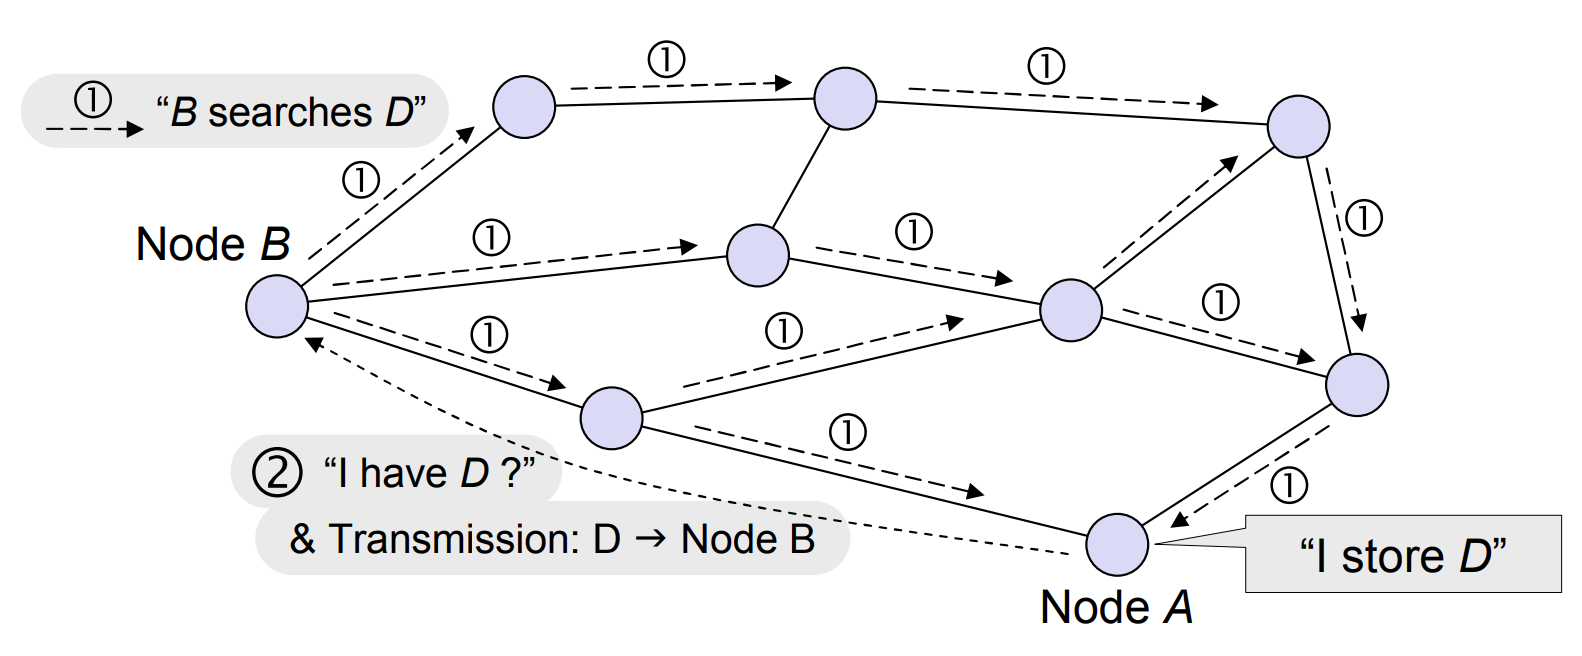
\includegraphics[width=0.7\textwidth]{images/02_flooding_search.png}
	\caption{\textbf{Flooding Search} : diffusion r\'ecursive de requ\^etes, puis retour des n\oe uds ayant la donn\'ee.}
	\label{fig:02_flooding_search}
\end{figure}

\newpage
\subsubsection*{3. Distributed Hash Tables (DHTs)}
Les DHTs (\emph{structured Peer-to-Peer systems}) structurent l'\emph{overlay} pour obtenir un compromis robuste : \(O(\log N)\) entr\'ees de routage par n\oe ud et \(O(\log N)\) \emph{hops} pour localiser une donn\'ee.

\begin{figure}[!ht]
	\centering
		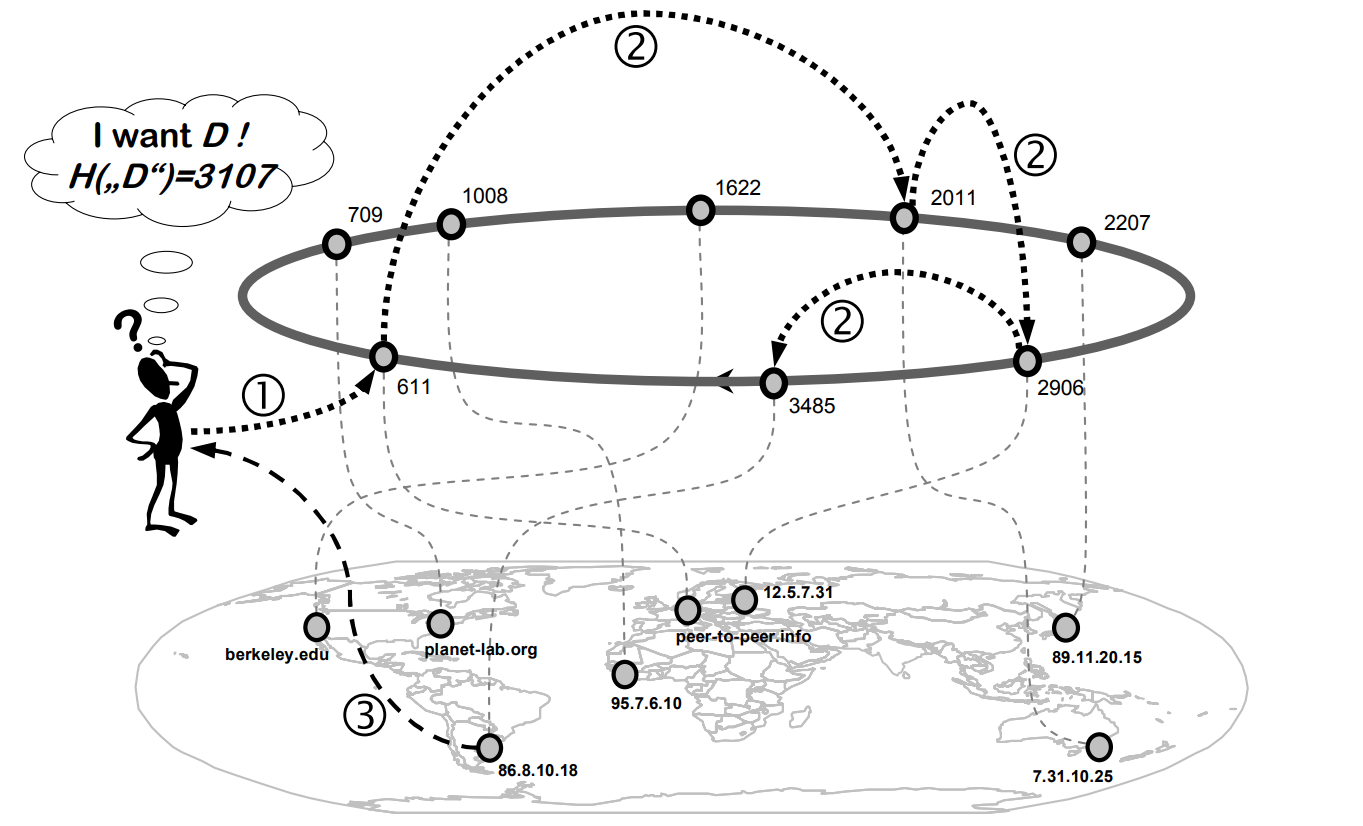
\includegraphics[width=0.7\textwidth]{images/04_dht_principle.png}
	\caption{\textbf{Distributed Hash Table} : routage structur\'e et efficace vers le n\oe ud responsable.}
	\label{fig:04_dht_principle}
\end{figure}

Les Figures~\ref{fig:01_central_server}, \ref{fig:02_flooding_search}, \ref{fig:04_dht_principle} et~\ref{fig:03_comparison_central_flooding_dht} montrent que les DHTs offrent le meilleur compromis entre co\^ut de recherche et co\^ut de stockage.

\begin{figure}[!ht]
	\centering
		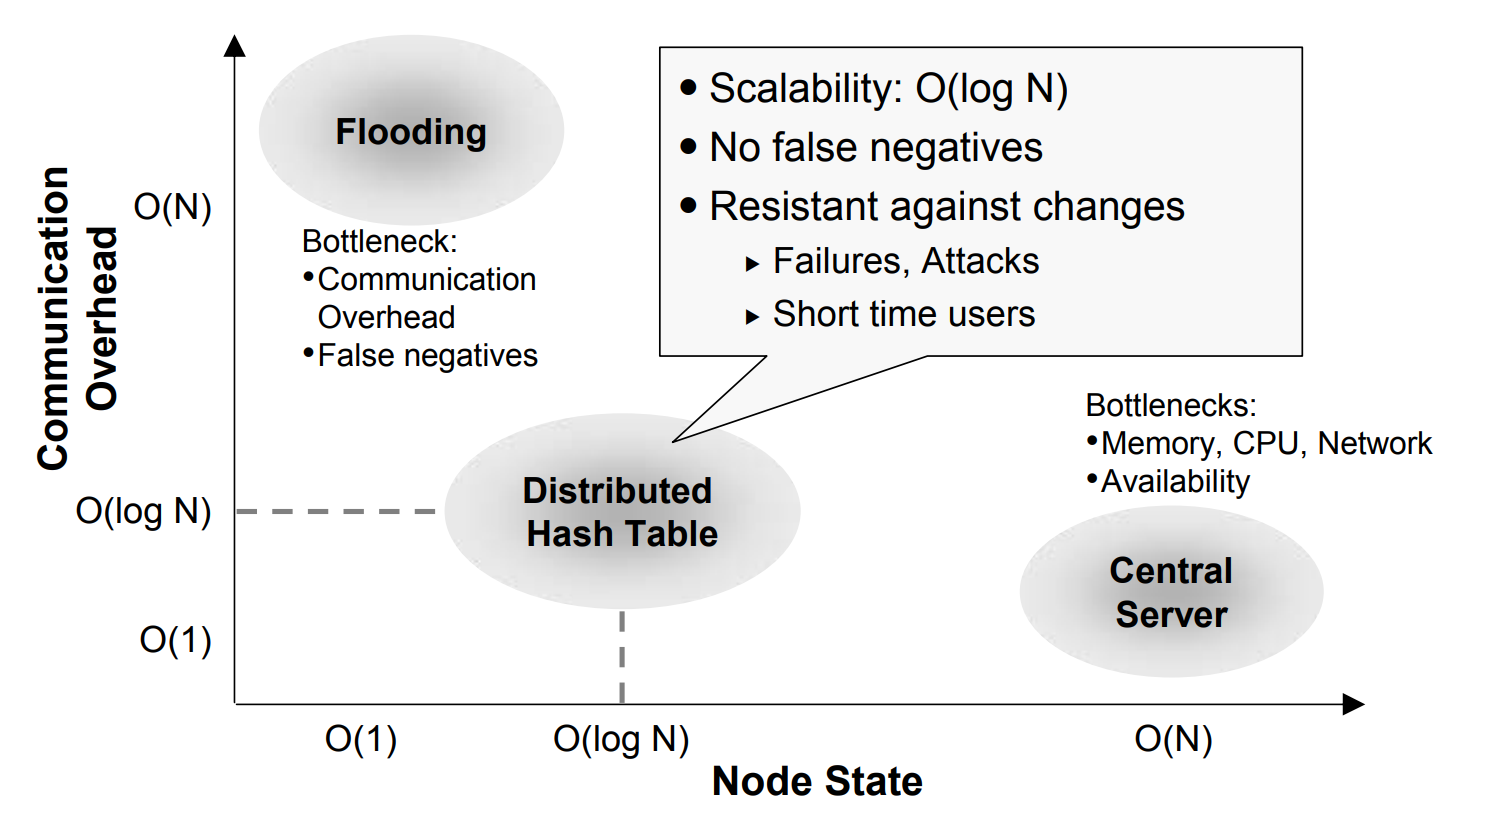
\includegraphics[width=0.7\textwidth]{images/03_comparison_central_flooding_dht.png}
\caption{Comparaison de la complexit\'e en termes d'effort de recherche (axe y) et de co\^ut de stockage par n\oe ud (axe x). Les goulots d'\'etranglement (\emph{bottlenecks}) ainsi que les caract\'eristiques sp\'ecifiques de chaque approche sont indiqu\'es.}
	\label{fig:03_comparison_central_flooding_dht}
\end{figure}

\newpage
\subsubsection{Fondamentaux des Distributed Hash Tables}

Une DHT associe chaque cl\'e \`a un n\oe ud responsable via un espace d'adressage logique et un routage d\'eterministe.

\subsubsection*{Gestion distribu\'ee des donn\'ees}
Chaque n\oe ud g\`ere une plage de cl\'es et conserve une \emph{partial view} du syst\`eme. Les messages sont relay\'es de n\oe ud en n\oe ud jusqu'\`a la destination.

\subsubsection*{Adressage dans les Distributed Hash Tables}
N\oe uds et donn\'ees partagent le m\^eme \emph{address space} logique (souvent tr\`es grand, p.~ex. \(0\) \`a \(2^{160}-1\)). Les IDs sont produits par une \emph{collision-resistant hash function}.

\begin{figure}[!ht]
	\centering
		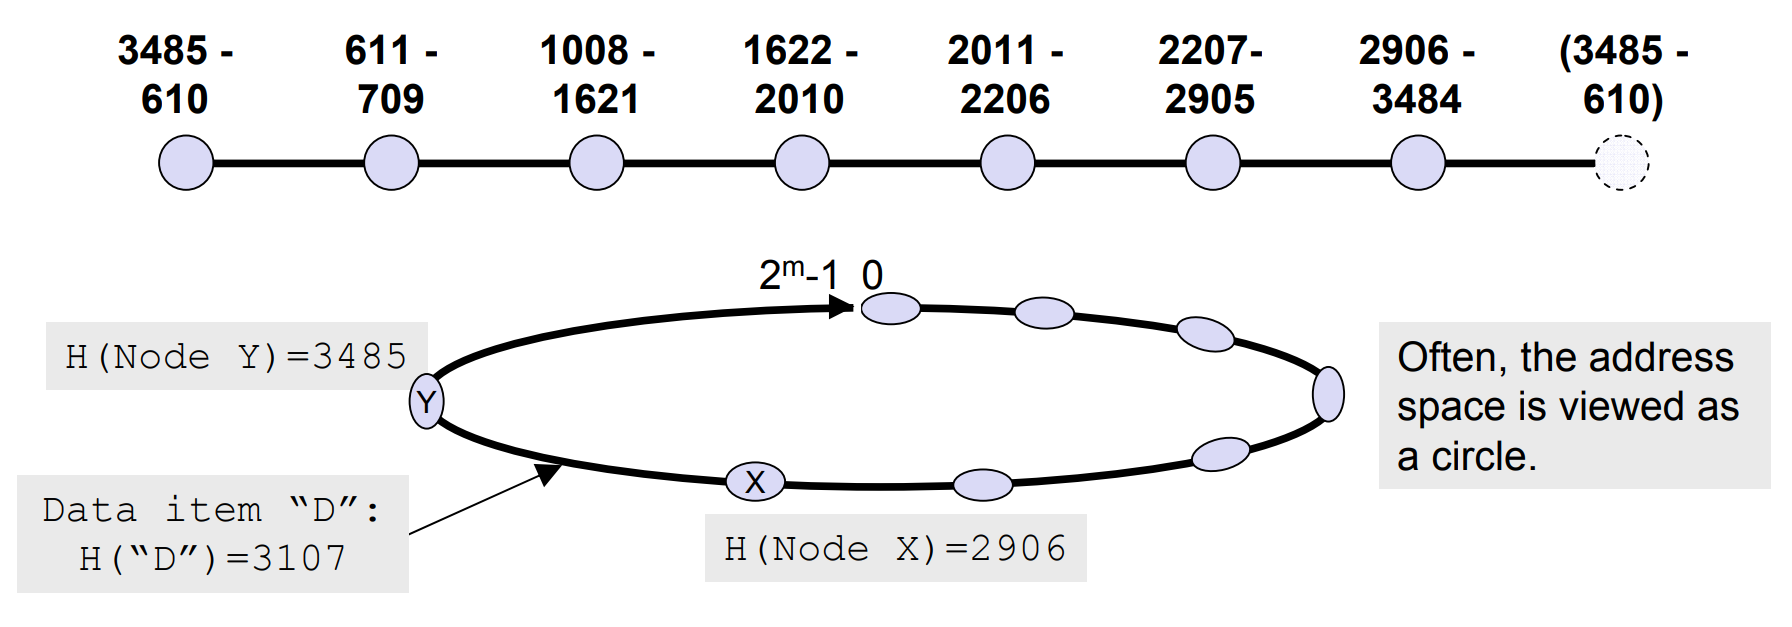
\includegraphics[width=0.7\textwidth]{images/05_a_linear_address_space_in_dht.png}
	\caption{Espace d'adressage lin\'eaire partitionn\'e entre pairs.}
	\label{fig:05_a_linear_address_space_in_dht}
\end{figure}

\begin{figure}[!ht]
	\centering
		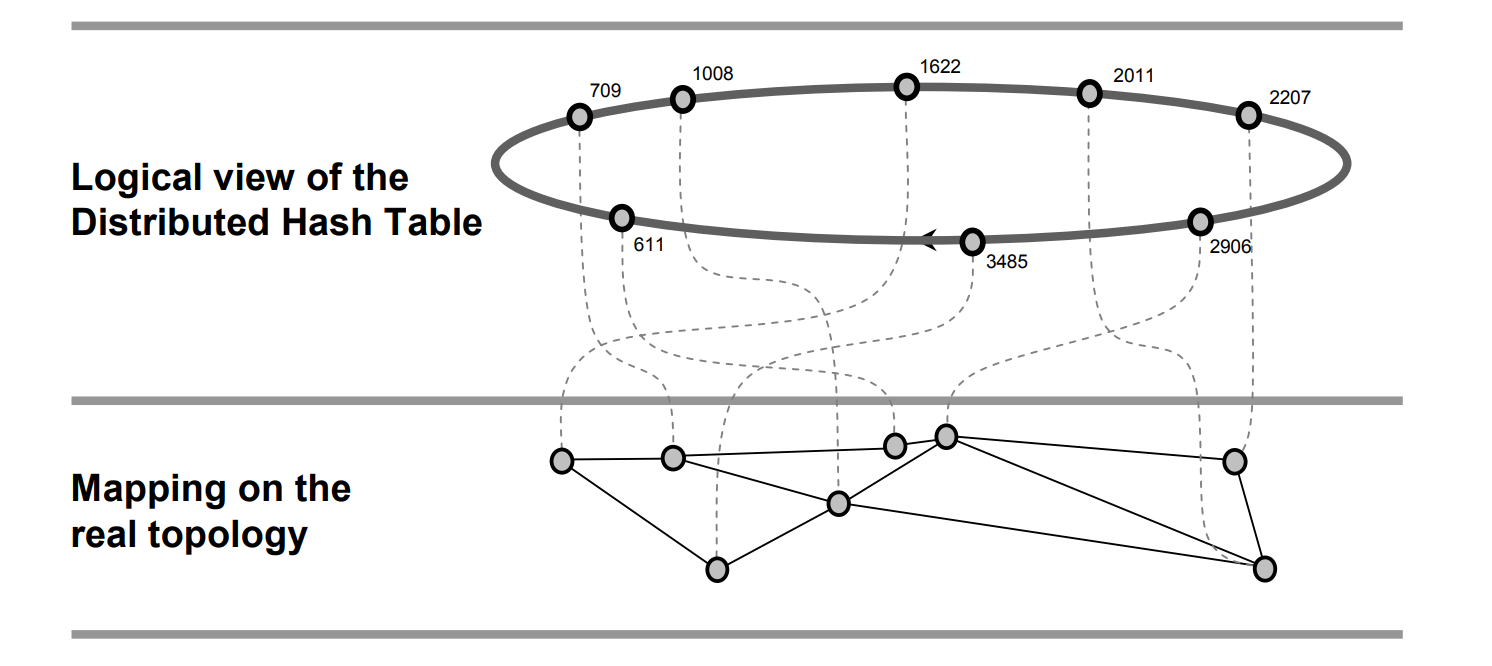
\includegraphics[width=0.7\textwidth]{images/06_underlay_view_of_dht.png}
	\caption{Vue logique de la DHT et vue du r\'eseau sous-jacent.}
	\label{fig:06_underlay_view_of_dht}
\end{figure}

\subsubsection*{Routage}
Chaque n\oe ud transmet vers un voisin plus proche de l'ID cible, ce qui r\'eduit progressivement la distance jusqu'au n\oe ud responsable en un \emph{small number of hops}.

\subsubsection*{M\'ethodes de stockage}
\textbf{Direct Storage} : la donn\'ee est copi\'ee sur le n\oe ud responsable (meilleure \emph{availability}, co\^ut plus \'elev\'e).

\textbf{Indirect Storage} : la DHT stocke un \emph{pointer} vers la donn\'ee (co\^ut r\'eduit, d\'ependance au n\oe ud source).

\begin{figure}[!ht]
	\centering
		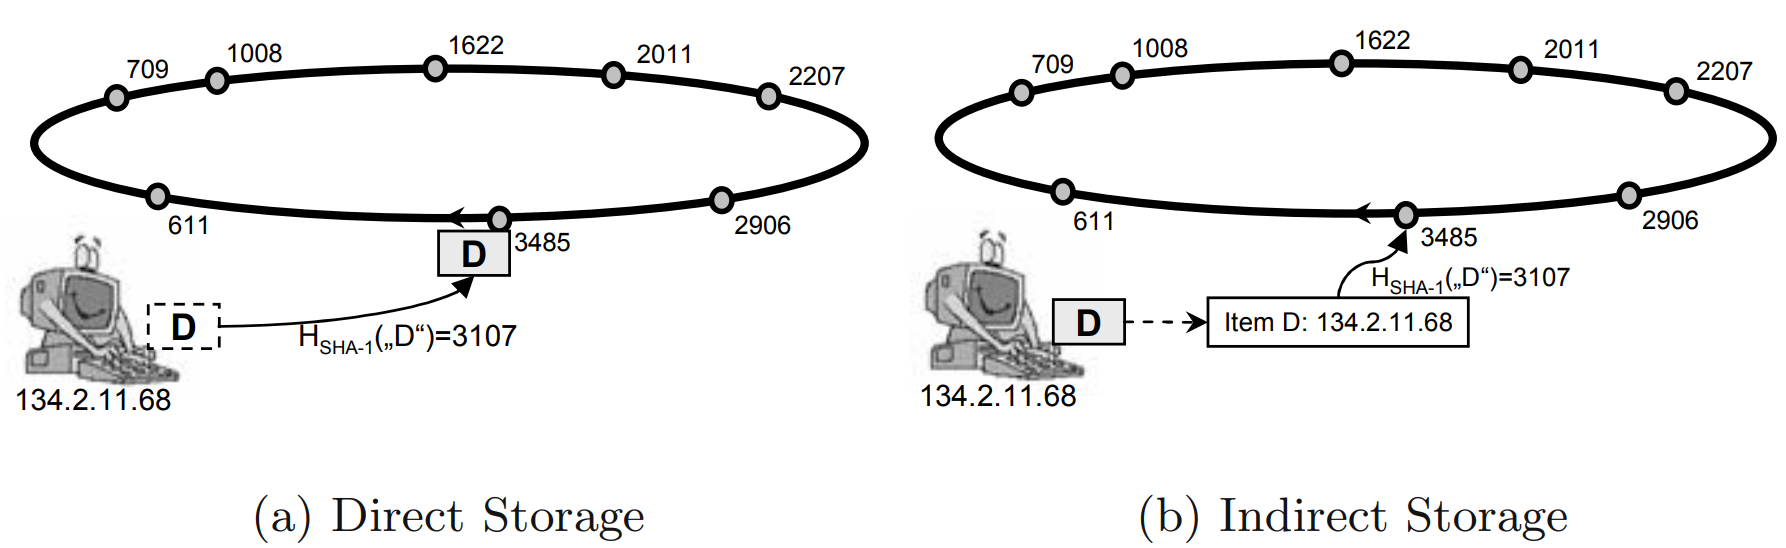
\includegraphics[width=0.7\textwidth]{images/07_direct_indirect_storage.png}
	\caption{Comparaison entre stockage direct et stockage indirect.}
	\label{fig:07_direct_indirect_storage}
\end{figure}

\subsubsection{M\'ecanismes des DHTs}

La robustesse d\'epend de la gestion du \emph{churn}, c'est-\`a-dire le taux de \emph{joins} et \emph{leaves} (arriv\'ees/d\'eparts) ainsi que les pannes fr\'equentes.

\subsubsection*{Arriv\'ee de n\oe uds}
L'entr\'ee d'un n\oe ud suit quatre \'etapes courtes :
\begin{enumerate}
\item \textbf{Bootstrap} : le nouveau pair contacte un n\oe ud existant qui sert d'\emph{entry point}.
\item \textbf{Address Assignment} : il re\c{c}oit sa partition dans le \emph{logical address space}.
\item \textbf{Routing Update} : les tables de routage sont ajust\'ees pour int\'egrer le nouveau pair.
\item \textbf{Data Transfer} : les paires \emph{(key, value)} devenues sa responsabilit\'e lui sont transf\'er\'ees.
\end{enumerate}

\subsubsection*{D\'efaillance de n\oe uds}
Deux approches coexistent : \emph{reactive recovery} (d\'etection pendant le routage, puis route alternative) et \emph{proactive recovery} (\emph{probes} p\'eriodiques, remplacement pr\'eventif des entr\'ees invalides). La \emph{replication} limite la perte de donn\'ees applicatives.

\subsubsection*{D\'epart de n\oe uds}
Un d\'epart volontaire (\emph{graceful leave}) facilite la migration imm\'ediate des donn\'ees vers le \emph{successor} et acc\'el\`ere la convergence des tables de routage. Il am\'eliore aussi la \emph{routing efficiency} et stabilise les m\'ecanismes de \emph{replication} et de \emph{load-balancing}.

\newpage
\subsubsection{Interfaces des DHTs}

\begin{figure}[h]
	\centering
		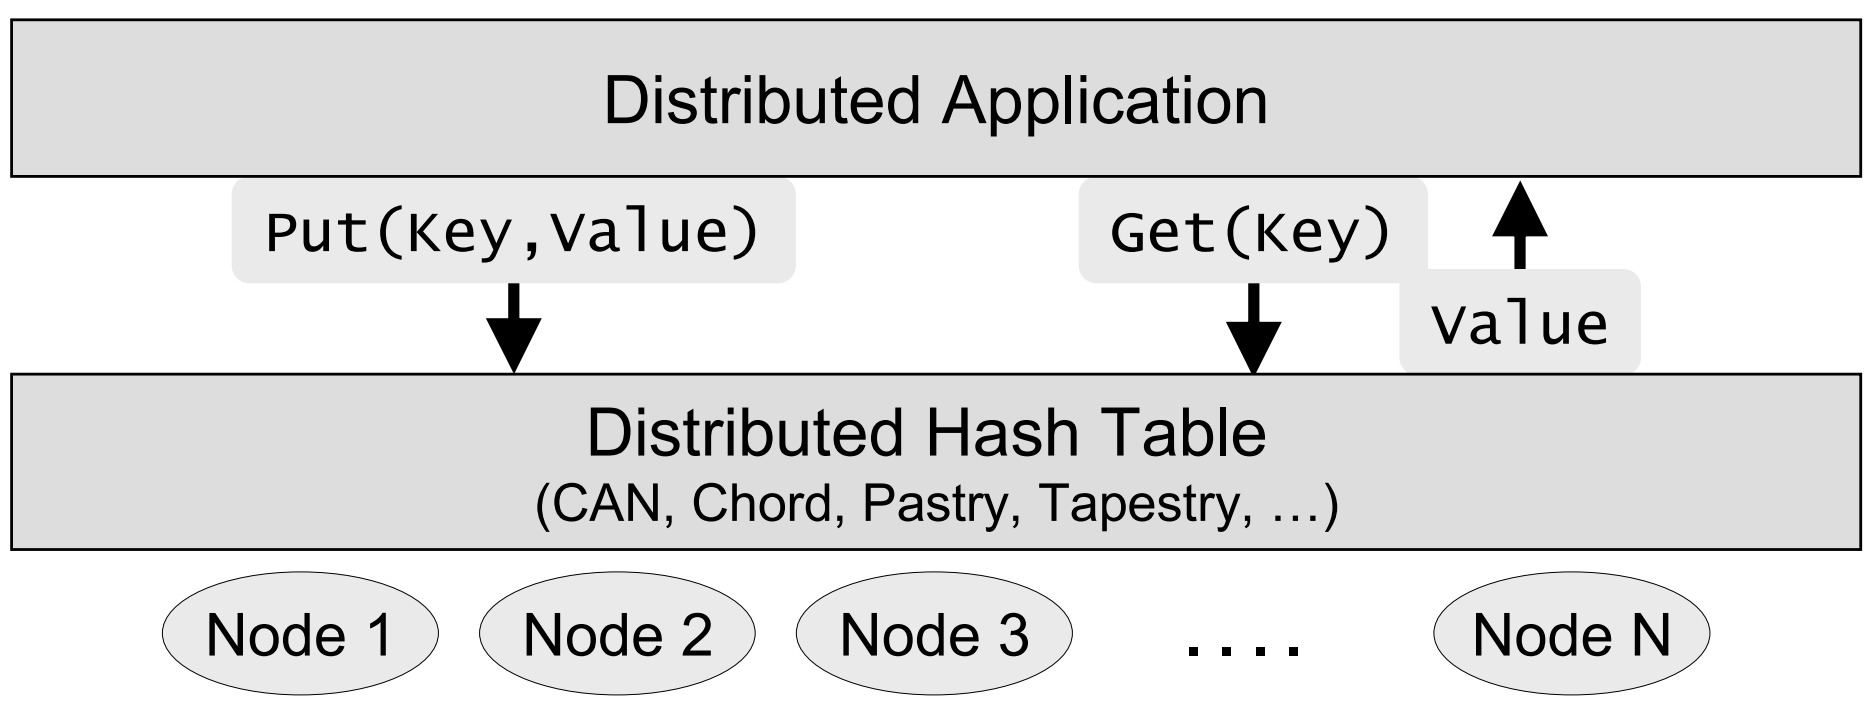
\includegraphics[width=0.5\textwidth]{images/08_interface_of_a_dht.png}
	\caption{Interface d'une Distributed Hash Table, typiquement \textsf{put}/\textsf{get}.}
	\label{fig:08_interface_of_a_dht}
\end{figure}

\subsubsection*{Interface de routage}
Interface \emph{stateless} orient\'ee messages : \texttt{send} livre vers un ID destination, \texttt{receive} remet les messages \`a l'application (\emph{delivery semantics}).
Cette \emph{stateless interface} se concentre sur la livraison de paquets bas\'es sur un ID logique plut\^ot que sur une adresse IP physique.

\subsubsection*{Interface de stockage}
Interface cl\'e-valeur : \texttt{put} \'ecrit la donn\'ee, \texttt{get} la r\'ecup\`ere. La couche g\`ere \emph{routing failures}, \emph{replication} et \emph{admission control}.
Cette couche ajoute de la complexit\'e car elle g\`ere la persistance et la fiabilit\'e des donn\'ees, comme une table de \emph{hash} distribu\'ee.

\subsubsection*{Interface Client}
Des h\^otes peuvent consommer le service DHT sans participer au routage de l'\emph{overlay} (mode \emph{client}).
Ce mode est utile quand on veut s\'eparer usage applicatif et participation au routage (fiabilit\'e, politiques d'\emph{access control}).

%\newpage
\subsubsection{Conclusions}

Les DHTs offrent une excellente \emph{scalability} sans point central, mais imposent des compromis entre efficacit\'e de routage, co\^ut de maintenance et r\'esilience au \emph{churn}.

\subsubsection*{D\'efis de conception}
\begin{itemize}
\item \textbf{Routing Efficiency} : qualit\'e du routage selon la structure des tables et la topologie.
\item \textbf{Management Overhead} : co\^ut de maintenance en continu.
\item \textbf{Churn} : impact des arriv\'ees/d\'eparts simultan\'es sur la stabilit\'e.
\end{itemize}

\subsubsection*{Limitations fondamentales}
\begin{itemize}
\item \textbf{Untrusted Environments} : r\'esistance difficile face aux n\oe uds malveillants et aux \emph{Byzantine faults}.
\item \textbf{Query Constraints} : \emph{fuzzy searches} et requ\^etes textuelles complexes peu adapt\'ees au mod\`ele par identifiants.
\end{itemize}

\newpage
\subsection{\'Etude de l'approche hi\'erarchis\'ee : HBase}

Les DHT repondent bien au \emph{lookup} en environnement dynamique, mais certaines applications exigent davantage de controle sur la coherence, la persistance et les performances de scan/ecriture. L'approche hi\'erarchis\'ee d'Apache HBase repond a ce besoin.

\subsubsection{Introduction au modele hierarchise}

HBase, construit sur HDFS (\emph{Hadoop Distributed File System}), est une base NoSQL distribu\'ee orient\'ee grands volumes. Contrairement aux DHT decentralisees, HBase suit un modele \emph{master-worker} avec \emph{range partitioning} : adressage d\'eterministe par \emph{row key}, scans sequentiels efficaces et coherence forte au niveau ligne.

\subsubsection{Fondamentaux architecturaux de HBase}

Le \emph{HBase Master} g\`ere le cluster (allocation des regions, equilibrage, d\'etection de pannes), tandis que les \emph{RegionServers} stockent les donn\'ees et executent les lectures/ecritures. Cette separation simplifie l'administration et le controle operationnel.

\subsubsection*{Mod\`ele de donn\'ees et espace d'adressage}

Le modele est oriente colonnes (tables, \emph{rows}, familles de colonnes). Les \emph{row keys} ordonnees lexicographiquement definissent l'espace d'adressage : excellent pour les scans et les requ\^etes par plages, mais sensible au design des cles.


\subsubsection{M\'ecanismes internes : partitionnement et gestion des pannes}

Deux mecanismes portent la scalabilite et la durabilite : partitionnement par regions et reaffectation apres panne.

\subsubsection*{Partitionnement horizontal par plages de cles}

Les tables sont decoupees en regions couvrant des plages continues de \emph{row keys}. Avec la croissance des donn\'ees, \emph{region splitting} repartit la charge entre RegionServers. Limite cl\'e : des cles monotones (ex.~timestamps) creent des \emph{hotspots} et du \emph{data skew} (\emph{storage skew}/\emph{access skew}).

Par rapport au \emph{consistent hashing} des DHT (distribution pseudo-aleatoire), HBase choisit un partitionnement d\'eterministe par ordre de cles.

\subsubsection*{Gestion des pannes et reaffectation}

En cas de panne d'un RegionServer, le Master (avec ZooKeeper) reassigne les regions. Avec le \emph{WAL} et HDFS, la reconstruction est robuste. Ce modele est centralise, contrairement a la reorganisation incrementale des DHT.


\subsubsection{Avantages et limites}

\textbf{Avantages.} Coherence forte en lecture/ecriture, tr\`es bonnes performances de scans sequentiels, et bonne scalabilite horizontale via \emph{region splitting} + ajout de RegionServers.

\textbf{Limites.} Forte sensibilite au schema de cles (risque de \emph{hotspot} et \emph{data skew}) et complexit\'e operationnelle elevee (HDFS, ZooKeeper, tuning et supervision du cluster).

\subsection{Conclusion et justification du choix architectural}

DHT et HBase repondent au meme objectif (stockage distribue a grande echelle) avec des choix opposes : decentralisation + \emph{consistent hashing} d'un cote, coordination centralisee + \emph{range partitioning} de l'autre.

\subsubsection*{Crit\`ere d'\'evaluation : gestion du data skew}

Le \emph{data skew} est determinant : HBase peut concentrer charge/stockage si les cles sont mal concues, alors que les DHT reduisent structurellement ce risque via une distribution pseudo-aleatoire des identifiants.

\subsubsection*{Motivation du choix}

Notre objectif est d'implementer un systeme totalement decentralise en anneau logique. Les DHT sont mieux alignees avec cet objectif (routage distribue, auto-organisation, joins/leaves, absence de maitre), tandis qu'une approche HBase deplacerait le projet vers l'ingenierie d'un cluster hierarchise.

\subsubsection*{Conclusion du choix}

HBase reste excellent pour des besoins de coherence forte et de scans massifs, mais pour nos objectifs pedagogiques/experimentaux, l'approche DHT est plus pertinente.
En consequence, nous retenons l'architecture DHT comme base de la suite du projet.
